\part{LAtex语法学习}
\section{Latex语法学习}
\subsection{伪代码}
\href{伪代码}{http://hustsxh.is-programmer.com/posts/38801.html}
\paragraph{algorithmic和algorithmics}
algorithmic和algorithmicx,这两个包很像,很多命令都是一样的,只是algorithmic的命令都是大写,algorithmicx的命令都是首字母大写,其他小写(EndFor两个大写)。下面是algorithmic的基本命令
还有algorithm2e,latex的与algorithm相关的包常用的有几个,algorithm、algorithmic、algorithmicx、algorithm2e,可以大致分成三类,或者说三个排版环境。最原始的是使用algorithm+algorithmic,这个最早出现,也是最难用的,需要自己定义一些指令。第二个排版环境是algorithm+algorithmicx,algorithmicx提供了一些宏定义和一些预定义好了的环境(layout),指令类似algorithmic。第三个是algorithm2e,只需要一个包,使用起来和编程的感觉很像,也是我更倾向使用的包。下面是使用algorithm2e的例子。[1]
\subsection{超链接}
需要的宏包 hyperref, 

\subsection{插入图片}

\subsection{tikz绘图}
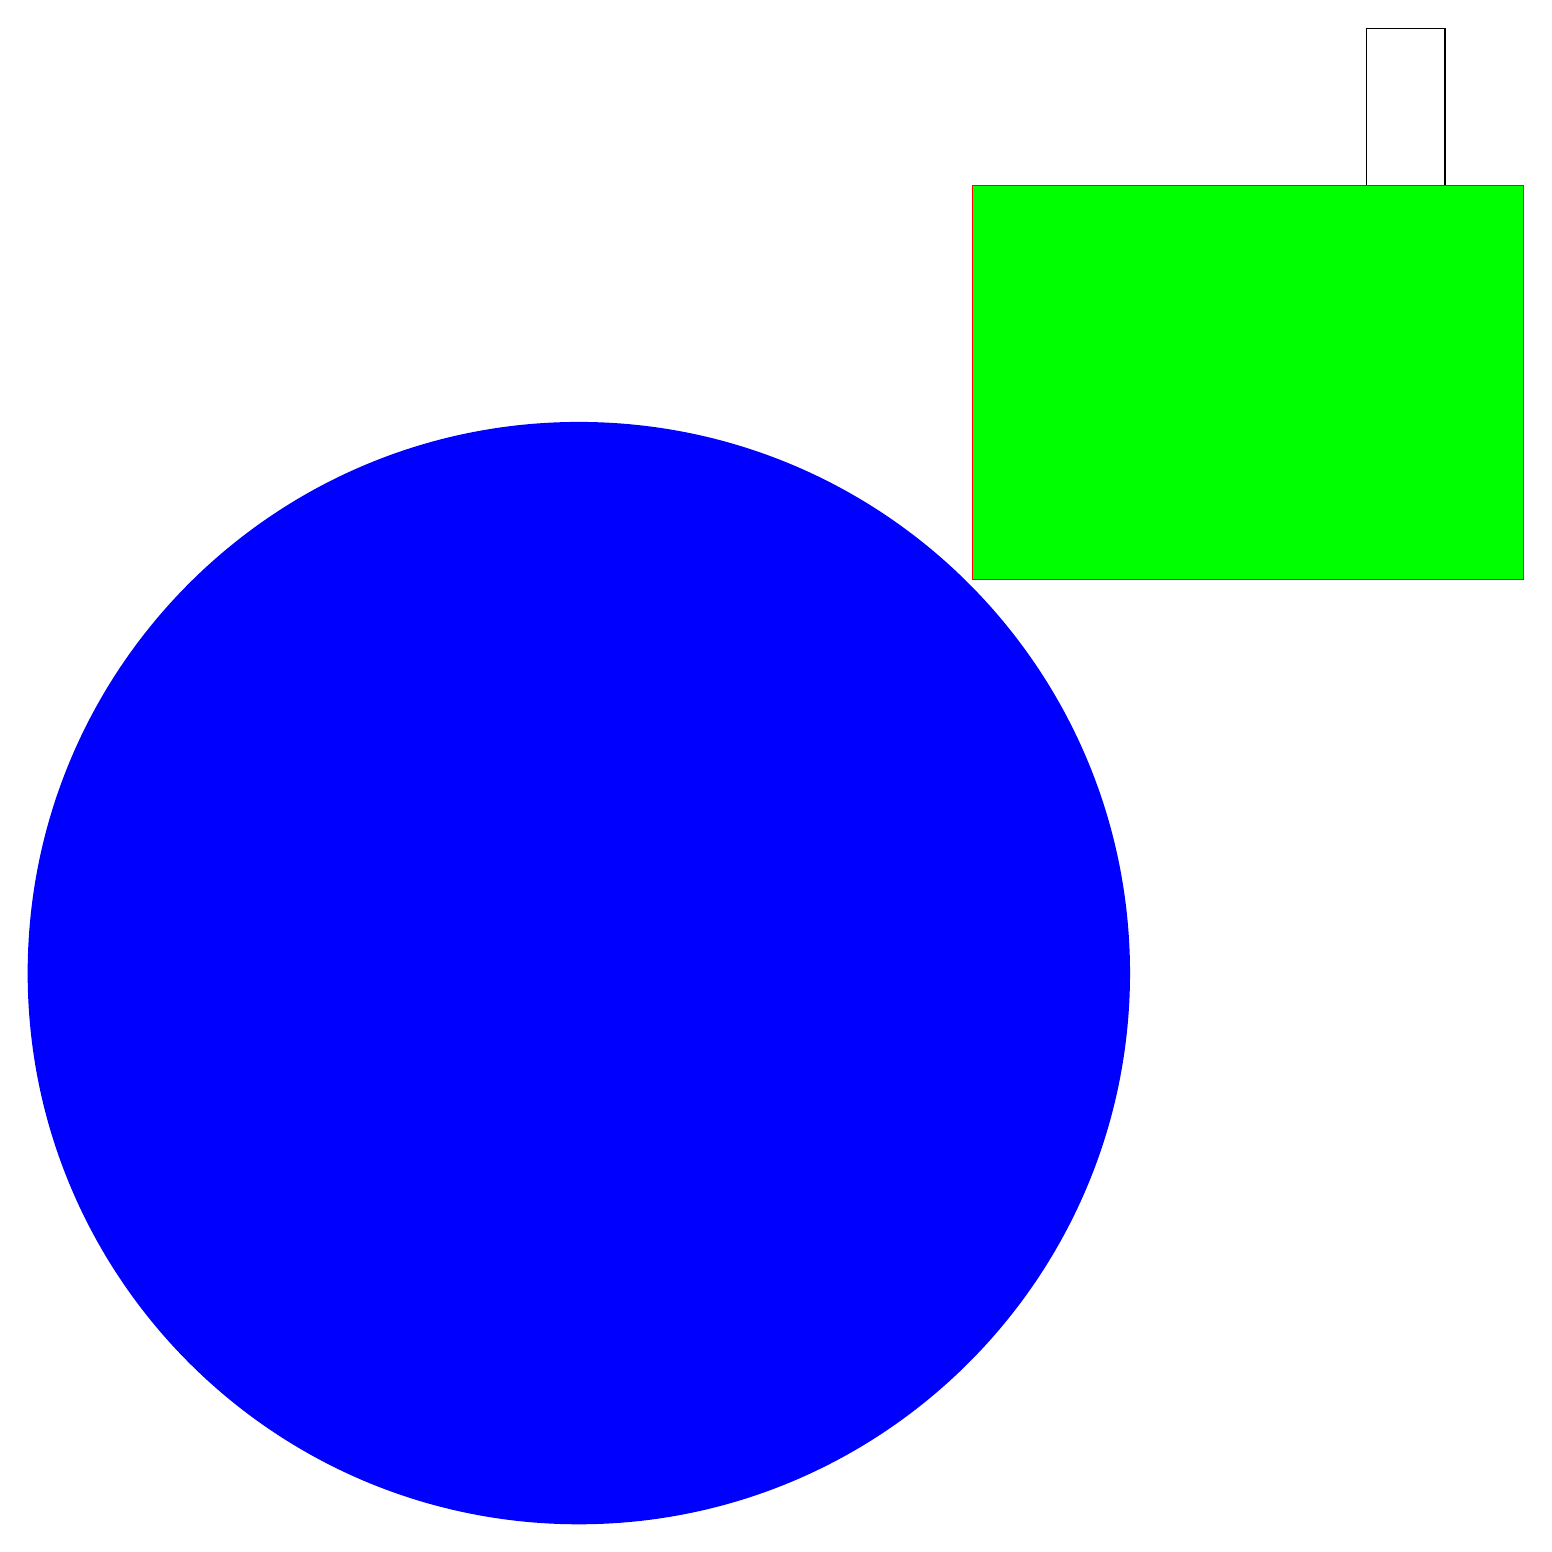
\begin{tikzpicture}
    \draw[red, -latex](0,0)--(5,5);
    \draw (5,5) rectangle (6,7);
    \filldraw[draw=red, fill=green] (0,0) rectangle (7,5);
    \fill[blue](-5,-5) circle [radius=7];
\end{tikzpicture}
% \mint{python}|test.py|		% 这里以Python语言为例。双竖线中是文件名
% \begin{minted}[mathescape,	% 中括号中的内容用于控制代码显示的格式,可以依照喜好修改
%                linenos,
%                numbersep=5pt,
%                gobble=2,
%                frame=lines,
%                framesep=2mm]{python}
% 	...		% 此处插入代码块,需要缩进
% \end{minted}
\tikzset{myarroe/.style={blue, thick,->}}
\begin{tikzpicture}
    \draw[myarroe] (0,0)--(5,5);
\end{tikzpicture}
\newpage
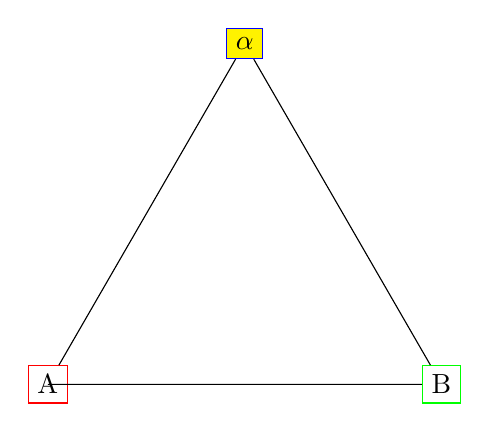
\begin{tikzpicture}
    \node[draw=red] (A) at (0,0) {A};
    \node[draw=green] (B) at (5,0) {B};
    \node[draw=blue,fill=yellow] (C) at (60:5) {$\alpha$};
    \filldraw (A.center) -- (B) -- (C) -- (A);
\end{tikzpicture}

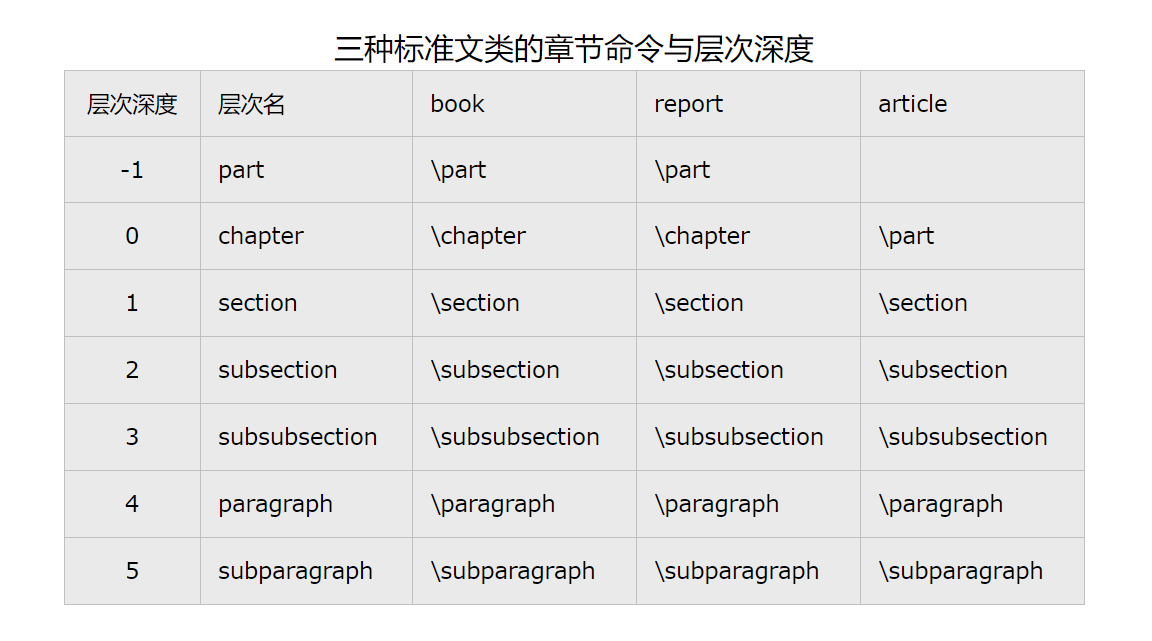
\includegraphics[width=\textwidth]{latex文档层次.PNG}



\begin{tikzpicture}
    \draw (0,0) node[left]{$A$} -- node[left]{$c$} (1,3)node[above] {$B$} --node[right]{$a$} (3,0) node[right]{$C$} -- node[below]{$b$}(0,0);
\end{tikzpicture}

\begin{lstlisting}[language={java}]
public class Main {
    public static void main(String[] args)
    {
        System.out.println("Hello,World");
    }
}
\end{lstlisting}
\section{Latex字体}
\subsection{Latex字母的三种类体}
正体 $\rm{R}$
\begin{lstlisting}
    $\rm{R}$
\end{lstlisting}
花体1 $\mathcal{R}$
\begin{lstlisting}
    $\mathcal{R}$
\end{lstlisting}
花体2 $\mathbb{R}$
\begin{lstlisting}
    $\mathbb{R}$
\end{lstlisting}
花体3 $\mathscr{R}$
\begin{lstlisting}
    $\mathscr{R}$
\end{lstlisting}